\chapter{Introduzione}

Quest’ultima parte del presente fascicolo ha lo scopo di caratterizzare l’aerodinamica del velivolo dell’Aviazione Generale {\bfseries JABIRU J450} \cite{prof:jabiru}.\\
In primo luogo, tramite l’applicazione della Teoria Globale del velivolo, saranno calcolati in funzione della quota, del peso e della velocità i parametri aerodinamici più significativi, quali coefficiente di portanza e resistenza indotta, velocità verticale e la deviazione impressa dalla corrente.
In seguito sarà determinato il carico aerodinamico lungo l’ala mediante l’implementazione del metodo ingegneristico di Schrenk. \\

\begin {figure} [h!]
\centering
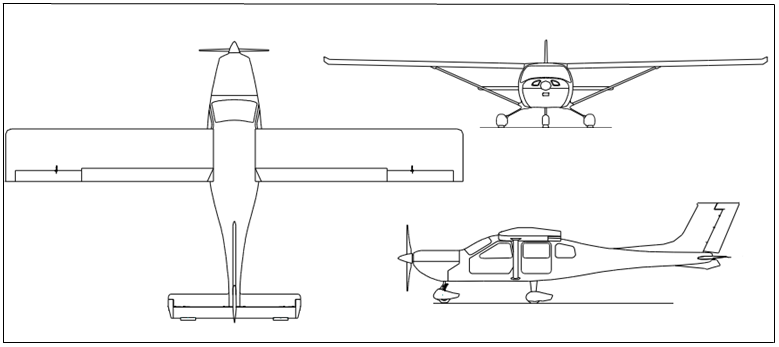
\includegraphics[height= 7cm ]{immagini/trittico.png}
\caption{\footnotesize Trittico JABIRU J450}
\label {fig:trittico}
\end {figure}
\noindent 

Il velivolo scelto per questa esercitazione è il {\bfseries JABIRU J450},un monomotore ad ala dritta prodotto dall’azienda indipendente australiana Jabiru Aircraft Pty Ltd. Il {\bfseries J450} è un velivolo quadriposto che si inserisce nel mercato come alternativa economica nell’ambito dei piccoli aeromobili da turismo, vantando costi di gestione molto contenuti.
Progettato per avere una tecnologia STOL ({\itshape Short Take Off and Landing}), il {\bfseries J450} fa parte dei cosiddetti “{\bfseries \itshape Kitplanes}”, ossia velivoli venduti sottoforma di kit e costruiti da persone non esperte nel settore.\\

Nelle tabelle  \ref{tab:tabella},  \ref{tab:tabellapeso},  \ref{tab:tabellaquote} sono elencanti i dati d'interesse del velivolo \\ \\ 

\begin{table} [!h]
\caption {Dati geometrici del velivolo J450}
\centering
\begin {tabular} {lp{8cm} l}
{\bfseries Dato }  & & { \bfseries Valore} \\ 
\hline \hline
Apertura Alare {\bfseries b}  & &  $ 9.140 m $ \\
\hline
Superficie Alare {\bfseries S} & & $11.15 m^2 $ \\
\hline
Allungamento alare {\bfseries \AR } & & $7.498 $ \\
\hline
Corda {\bfseries c } & & $ 1.22 m $ \\
\hline
Fattore di Oswald {\bfseries e } & & $ 0.69 $ \\
\hline
\end{tabular}
\label{tab:tabella}
\end{table}

\noindent \\ \\ \\ \\

\begin{table} [!h]
\caption {Pesi e velocità caratteristiche del velivolo J450}
\centering
\begin {tabular} {lp{6cm} l}
{\bfseries Dato }  & & { \bfseries Valore} \\ 
\hline \hline
Velocità di crociera {\bfseries $V_c$}  & &  $59.16 m/s $ \\
\hline
Velocità massima {\bfseries $V_{max}$}  & &   $64.30 m/s $ \\
\hline
Velocità di Stallo {\itshape full flap} {\bfseries $V_{sf}$} & & $23.15  m/s$ \\
\hline
Velocità di Stallo {\itshape no flap} {\bfseries $V_{sc}$} & & $28.30 m/s$ \\
\hline
Peso massimo al decollo {\bfseries $W_{TO_{max}}$} & & $700 Kg $ \\
\hline
Peso a vuoto {\bfseries $W_{OE}$} & & $340 Kg $ \\
\hline
Massimo peso {\itshape payload} {\bfseries $W_{PL}$} & & $370 Kg $ \\
\hline
\end{tabular}
\label{tab:tabellapeso}
\end{table}

\noindent \\ \\ \\ \\


\begin{table} [!h]
\caption {Quote e densità}
\centering
\begin {tabular} {lp{5cm} l}
{\bfseries Dato }  & & { \bfseries Valore} \\ 
\hline \hline
Quota di tangenza {\itshape Service Ceiling}  & &  $ 4570 m $ \\
\hline
Densità al livello del mare  {\bfseries ${\rho}_{SL}$}  & & $1.225  Kg/m^3$ \\
\hline
Densità alla quota di tangenza  {\bfseries ${\rho}_{C}$}  & & $0.66945  Kg/m^3$ \\
\hline
\end{tabular}
\label{tab:tabellaquote}
\end{table}


